\documentclass[]{standalone}
\usepackage{tikz}
\begin{document}
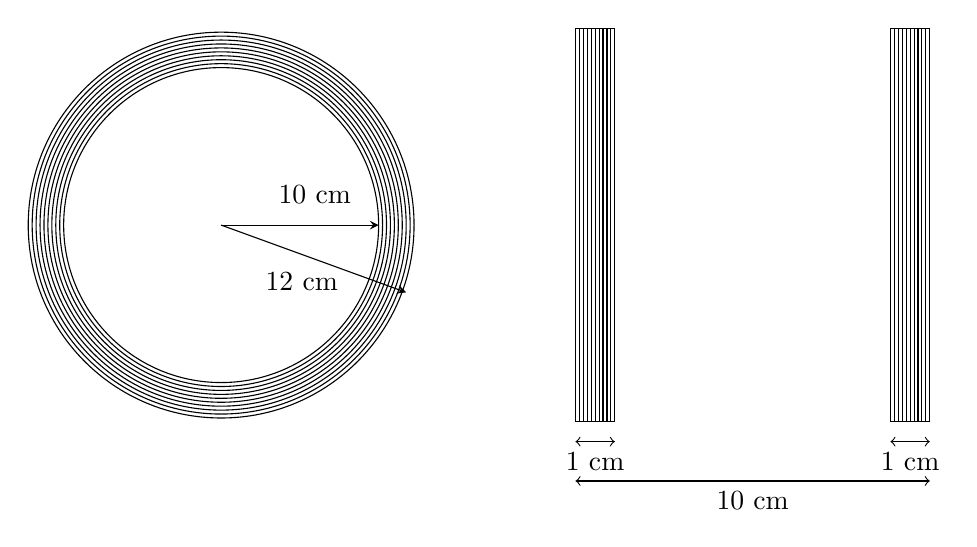
\begin{tikzpicture}
	\foreach \index in {2,2.05,2.1,...,2.5}
	{
	\draw (0,0) circle (\index cm);
}
	\draw[-stealth] (0:0) -- (0:2) node at (18:1.25) {10 cm};
	\draw[-stealth] (0:0) -- (-20:2.5) node at (-35:1.25) {12 cm};

	\draw (4.5,2.5) rectangle (5,-2.5);
	\draw[<->] (4.5,-2.75) -- (5,-2.75) node at (4.75,-3) {1 cm};
	\draw (8.5,2.5) rectangle (9,-2.5);
	\draw[<->] (8.5,-2.75) -- (9,-2.75) node at (8.75,-3) {1 cm};
	\foreach \index in {8.5,8.55,8.6,...,9.0}
	{
		\draw (\index, 2.5) -- (\index, -2.5);
		\draw (\index-4, 2.5) -- (\index-4, -2.5);
	}
	\draw[<->] (4.5,-3.25) -- (9,-3.25) node at (6.75, -3.5) {10 cm};;
\end{tikzpicture}



\end{document}
